\documentclass{standalone}
\usepackage{tikz}
\usetikzlibrary{patterns, positioning}
\usepackage[sfdefault]{ClearSans} %% option 'sfdefault' activates Clear Sans as the default text font
\usepackage[T1]{fontenc}

\begin{document}
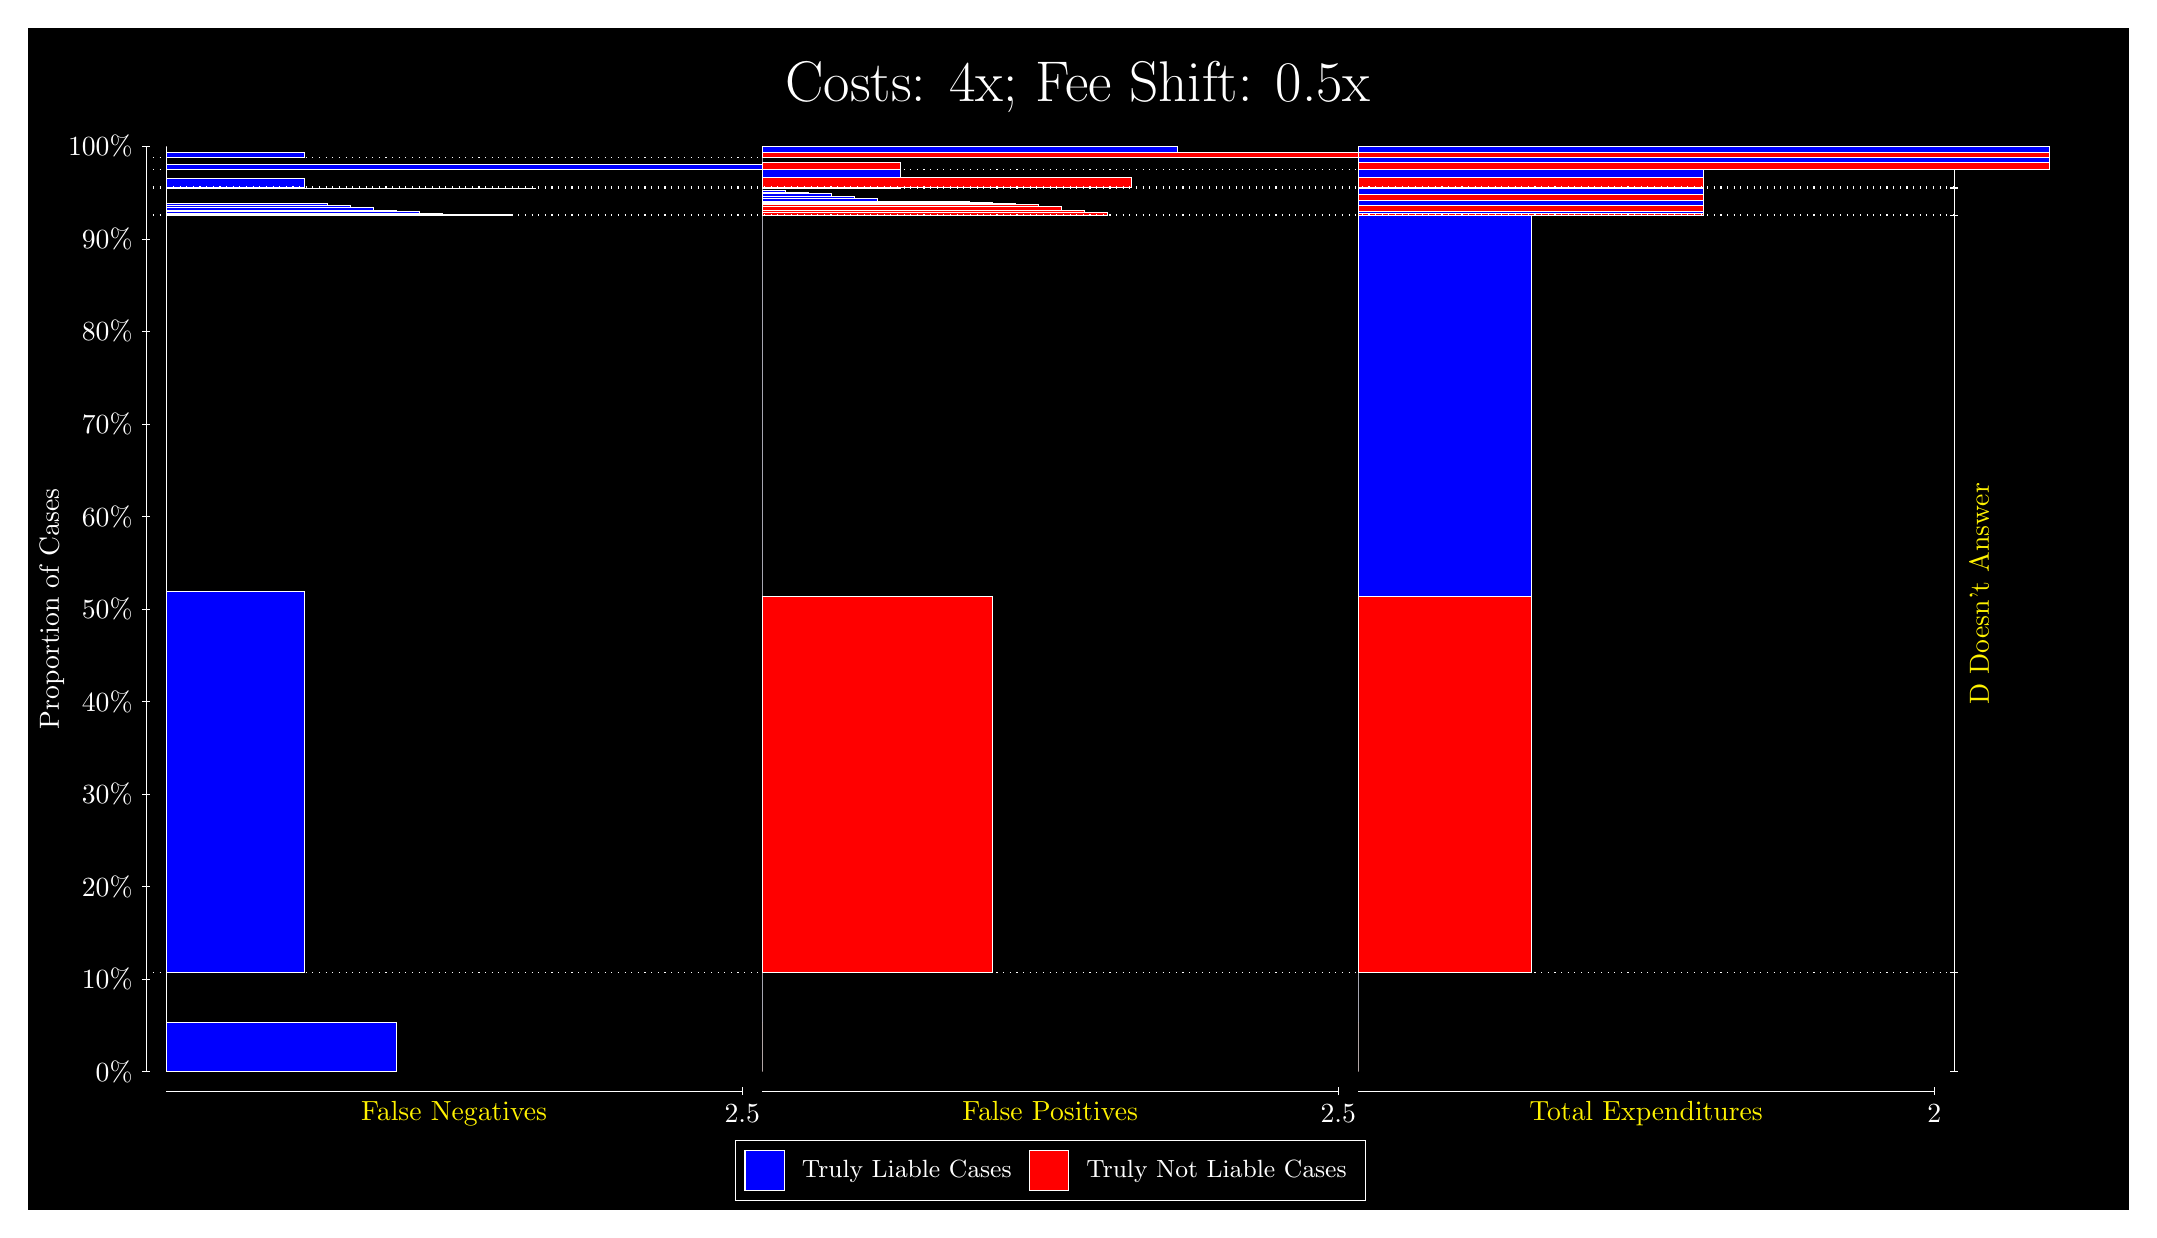
\begin{tikzpicture}
\draw[fill=black] (0,0) rectangle (26.667,15);
\draw[text=white] (0,13.5) rectangle (26.667,15) node[midway] {\huge Costs: 4x; Fee Shift: 0.5x};
\draw[white, very thin] (1.5,1.75) -- (1.5,13.5);
\node[rotate=90, text=white, anchor=center] at (0.3, 7.625) {Proportion of Cases};
\draw[white, very thin] (1.45,1.75) -- (1.55,1.75);
\node[text=white, anchor=east] at (1.45, 1.75) {0\%};
\draw[white, very thin] (1.45,2.925) -- (1.55,2.925);
\node[text=white, anchor=east] at (1.45, 2.925) {10\%};
\draw[white, very thin] (1.45,4.1) -- (1.55,4.1);
\node[text=white, anchor=east] at (1.45, 4.1) {20\%};
\draw[white, very thin] (1.45,5.275) -- (1.55,5.275);
\node[text=white, anchor=east] at (1.45, 5.275) {30\%};
\draw[white, very thin] (1.45,6.45) -- (1.55,6.45);
\node[text=white, anchor=east] at (1.45, 6.45) {40\%};
\draw[white, very thin] (1.45,7.625) -- (1.55,7.625);
\node[text=white, anchor=east] at (1.45, 7.625) {50\%};
\draw[white, very thin] (1.45,8.8) -- (1.55,8.8);
\node[text=white, anchor=east] at (1.45, 8.8) {60\%};
\draw[white, very thin] (1.45,9.975) -- (1.55,9.975);
\node[text=white, anchor=east] at (1.45, 9.975) {70\%};
\draw[white, very thin] (1.45,11.15) -- (1.55,11.15);
\node[text=white, anchor=east] at (1.45, 11.15) {80\%};
\draw[white, very thin] (1.45,12.325) -- (1.55,12.325);
\node[text=white, anchor=east] at (1.45, 12.325) {90\%};
\draw[white, very thin] (1.45,13.5) -- (1.55,13.5);
\node[text=white, anchor=east] at (1.45, 13.5) {100\%};

\draw[white, very thin] (24.457,1.75) -- (24.457,13.5);
\draw[white, very thin] (24.407,1.75) -- (24.507,1.75);
\node[anchor=west] at (24.407, 1.75) {};
\draw[white, very thin] (24.407,3.0078) -- (24.507,3.0078);
\node[anchor=west] at (24.407, 3.0078) {};
\draw[white, very thin] (24.407,12.628) -- (24.507,12.628);
\node[anchor=west] at (24.407, 12.628) {};
\draw[white, very thin] (24.407,12.964) -- (24.507,12.964);
\node[anchor=west] at (24.407, 12.964) {};
\draw[white, very thin] (24.407,12.984) -- (24.507,12.984);
\node[anchor=west] at (24.407, 12.984) {};
\draw[white, very thin] (24.407,13.208) -- (24.507,13.208);
\node[anchor=west] at (24.407, 13.208) {};
\draw[white, very thin] (24.407,13.355) -- (24.507,13.355);
\node[anchor=west] at (24.407, 13.355) {};
\draw[white, very thin] (24.407,13.5) -- (24.507,13.5);
\node[anchor=west] at (24.407, 13.5) {};

\draw[white, very thin, fill=blue] (1.75,1.75) rectangle (4.6775,2.3789);
\draw[white, very thin, fill=red] (1.75,2.3789) rectangle (1.75,3.0078);
\draw[white, very thin, fill=blue] (1.75,3.0078) rectangle (3.5065,7.8469);
\draw[white, very thin, fill=red] (1.75,7.8469) rectangle (1.75,12.628);
\draw[white, very thin, fill=blue] (1.75,12.628) rectangle (6.1413,12.631);
\draw[white, very thin, fill=blue] (1.75,12.631) rectangle (5.8486,12.635);
\draw[white, very thin, fill=blue] (1.75,12.635) rectangle (5.5558,12.643);
\draw[white, very thin, fill=blue] (1.75,12.643) rectangle (5.2631,12.65);
\draw[white, very thin, fill=blue] (1.75,12.65) rectangle (4.9703,12.67);
\draw[white, very thin, fill=blue] (1.75,12.67) rectangle (4.6775,12.687);
\draw[white, very thin, fill=blue] (1.75,12.687) rectangle (4.3848,12.728);
\draw[white, very thin, fill=blue] (1.75,12.728) rectangle (4.092,12.756);
\draw[white, very thin, fill=blue] (1.75,12.756) rectangle (3.7993,12.783);
\draw[white, very thin, fill=red] (1.75,12.783) rectangle (1.75,12.964);
\draw[white, very thin, fill=blue] (1.75,12.964) rectangle (6.4341,12.973);
\draw[white, very thin, fill=red] (1.75,12.973) rectangle (1.75,12.984);
\draw[white, very thin, fill=blue] (1.75,12.984) rectangle (3.5065,13.089);
\draw[white, very thin, fill=red] (1.75,13.089) rectangle (1.75,13.208);
\draw[white, very thin, fill=blue] (1.75,13.208) rectangle (9.9471,13.271);
\draw[white, very thin, fill=red] (1.75,13.271) rectangle (1.75,13.355);
\draw[white, very thin, fill=blue] (1.75,13.355) rectangle (3.5065,13.429);
\draw[white, very thin, fill=red] (1.75,13.429) rectangle (1.75,13.5);
\draw[white, very thin, fill=red] (9.3189,1.75) rectangle (9.3189,2.3789);
\draw[white, very thin, fill=blue] (9.3189,2.3789) rectangle (9.3189,3.0078);
\draw[white, very thin, fill=red] (9.3189,3.0078) rectangle (12.246,7.7884);
\draw[white, very thin, fill=blue] (9.3189,7.7884) rectangle (9.3189,12.628);
\draw[white, very thin, fill=red] (9.3189,12.628) rectangle (13.71,12.657);
\draw[white, very thin, fill=red] (9.3189,12.657) rectangle (13.417,12.69);
\draw[white, very thin, fill=red] (9.3189,12.69) rectangle (13.125,12.74);
\draw[white, very thin, fill=red] (9.3189,12.74) rectangle (12.832,12.759);
\draw[white, very thin, fill=red] (9.3189,12.759) rectangle (12.539,12.783);
\draw[white, very thin, fill=red] (9.3189,12.783) rectangle (12.246,12.79);
\draw[white, very thin, fill=red] (9.3189,12.79) rectangle (11.954,12.799);
\draw[white, very thin, fill=red] (9.3189,12.799) rectangle (11.661,12.804);
\draw[white, very thin, fill=red] (9.3189,12.804) rectangle (11.368,12.808);
\draw[white, very thin, fill=blue] (9.3189,12.808) rectangle (10.783,12.836);
\draw[white, very thin, fill=blue] (9.3189,12.836) rectangle (10.49,12.863);
\draw[white, very thin, fill=blue] (9.3189,12.863) rectangle (10.197,12.904);
\draw[white, very thin, fill=blue] (9.3189,12.904) rectangle (9.9044,12.921);
\draw[white, very thin, fill=blue] (9.3189,12.921) rectangle (9.6116,12.942);
\draw[white, very thin, fill=blue] (9.3189,12.942) rectangle (9.3189,12.964);
\draw[white, very thin, fill=red] (9.3189,12.964) rectangle (11.075,12.974);
\draw[white, very thin, fill=blue] (9.3189,12.974) rectangle (9.3189,12.984);
\draw[white, very thin, fill=red] (9.3189,12.984) rectangle (14.003,13.103);
\draw[white, very thin, fill=blue] (9.3189,13.103) rectangle (11.075,13.208);
\draw[white, very thin, fill=red] (9.3189,13.208) rectangle (11.075,13.292);
\draw[white, very thin, fill=blue] (9.3189,13.292) rectangle (9.3189,13.355);
\draw[white, very thin, fill=red] (9.3189,13.355) rectangle (17.516,13.426);
\draw[white, very thin, fill=blue] (9.3189,13.426) rectangle (14.588,13.5);
\draw[white, very thin, fill=red] (16.888,1.75) rectangle (16.888,2.3789);
\draw[white, very thin, fill=blue] (16.888,2.3789) rectangle (16.888,3.0078);
\draw[white, very thin, fill=red] (16.888,3.0078) rectangle (19.083,7.7884);
\draw[white, very thin, fill=blue] (16.888,7.7884) rectangle (19.083,12.628);
\draw[white, very thin, fill=red] (16.888,12.628) rectangle (21.279,12.651);
\draw[white, very thin, fill=blue] (16.888,12.651) rectangle (21.279,12.671);
\draw[white, very thin, fill=red] (16.888,12.671) rectangle (21.279,12.746);
\draw[white, very thin, fill=blue] (16.888,12.746) rectangle (21.279,12.812);
\draw[white, very thin, fill=red] (16.888,12.812) rectangle (21.279,12.895);
\draw[white, very thin, fill=blue] (16.888,12.895) rectangle (21.279,12.964);
\draw[white, very thin, fill=red] (16.888,12.964) rectangle (21.279,12.974);
\draw[white, very thin, fill=blue] (16.888,12.974) rectangle (21.279,12.984);
\draw[white, very thin, fill=red] (16.888,12.984) rectangle (21.279,13.103);
\draw[white, very thin, fill=blue] (16.888,13.103) rectangle (21.279,13.208);
\draw[white, very thin, fill=red] (16.888,13.208) rectangle (25.67,13.292);
\draw[white, very thin, fill=blue] (16.888,13.292) rectangle (25.67,13.355);
\draw[white, very thin, fill=red] (16.888,13.355) rectangle (25.67,13.426);
\draw[white, very thin, fill=blue] (16.888,13.426) rectangle (25.67,13.5);
\draw[white, dotted] (1.5,3.0078) -- (24.457,3.0078);
\draw[white, dotted] (1.5,12.628) -- (24.457,12.628);
\draw[white, dotted] (1.5,12.964) -- (24.457,12.964);
\draw[white, dotted] (1.5,12.984) -- (24.457,12.984);
\draw[white, dotted] (1.5,13.208) -- (24.457,13.208);
\draw[white, dotted] (1.5,13.355) -- (24.457,13.355);
\draw[white, very thin] (1.75,1.5) -- (9.0689,1.5);
\node[text=yellow, anchor=north] at (5.4094, 1.5) {False Negatives};
\draw[white, very thin] (9.0689,1.45) -- (9.0689,1.55);
\node[text=white, anchor=north] at (9.0689, 1.45) {2.5};

\draw[white, very thin] (9.3189,1.5) -- (16.638,1.5);
\node[text=yellow, anchor=north] at (12.978, 1.5) {False Positives};
\draw[white, very thin] (16.638,1.45) -- (16.638,1.55);
\node[text=white, anchor=north] at (16.638, 1.45) {2.5};

\draw[white, very thin] (16.888,1.5) -- (24.207,1.5);
\node[text=yellow, anchor=north] at (20.547, 1.5) {Total Expenditures};
\draw[white, very thin] (24.207,1.45) -- (24.207,1.55);
\node[text=white, anchor=north] at (24.207, 1.45) {2};


\node[text=yellow, centered, rotate=90] at (24.777, 7.8177) {D Doesn't Answer};






\draw (12.978300999999998,1.5) node[draw=none] (baseCoordinate) {};
\begin{scope}[align=center]
        \matrix[scale=0.5, draw=white, below=0.5cm of baseCoordinate, nodes={draw}, column sep=0.1cm]{
            \node[rectangle, draw, minimum width=0.5cm, minimum height=0.5cm, fill=blue] {}; &
            \node[draw=none, font=\small, text=white] (B) {Truly Liable Cases}; &
            \node[rectangle, draw, minimum width=0.5cm, minimum height=0.5cm, fill=red] {}; &
            \node[draw=none, font=\small, text=white] (B) {Truly Not Liable Cases}; \\
            };
\end{scope}

\end{tikzpicture}
\end{document}